\documentclass[border=2pt]{standalone}
\usepackage{tikz}
\usetikzlibrary{datavisualization.formats.functions,datavisualization.polar}
\begin{document}
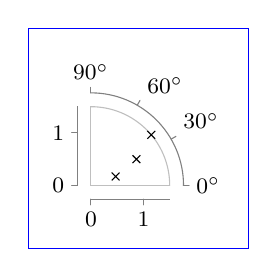
\begin{tikzpicture}
  \draw[blue,line width=.2pt] (-.8,-.8) rectangle (2,2);
  \datavisualization [scientific polar axes={clean,0 to 90},
    angle axis={ticks={step=30}},radius axis={length=1cm,ticks={step=1}},visualize as scatter]
    data point [angle=20,radius=.5]
    data point [angle=30,radius=1]
    data point [angle=40,radius=1.5];
\end{tikzpicture}
\end{document}
